% LTeX: language=it

\section{Onde elettromagnetiche}

Le onde elettromagnetiche sono il risultato della propagazione simultanea di un campo magnetico $\vec{B}$ e di un campo elettrico $\vec{E}$, perpendicolari tra loro.
Il primo a provare a l'esistenza di queste onde fu il fisico Hertz, che provocando una scintilla, riuscì a produrne un altra in due punti diversi della stanza.
La prima scintilla aveva prodotto un onda elettromagnetica.

\begin{figure}[H]
    \centering

    % https://tikz.net/electromagnetic_wave/
    % Electromagnetic wave - colored
    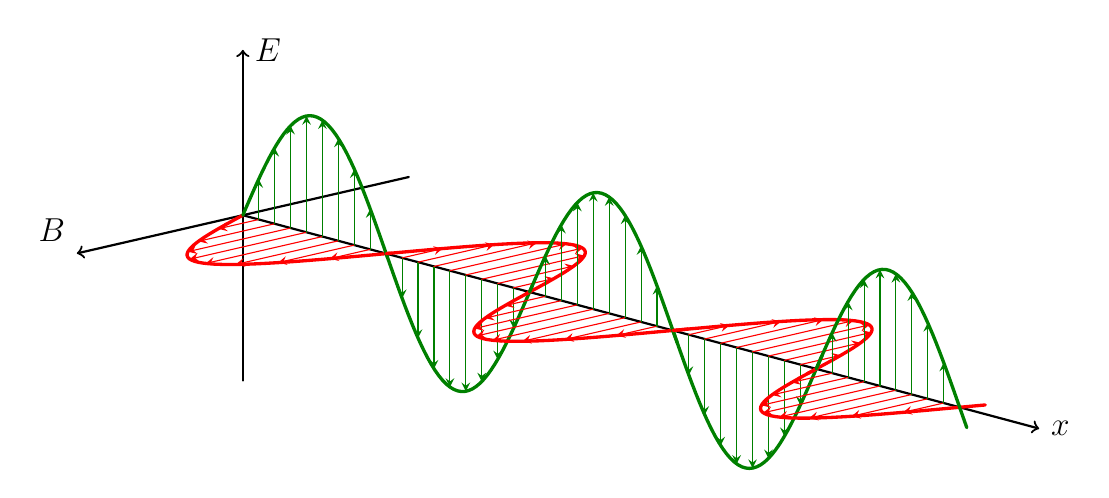
\begin{tikzpicture}[x=(-15:1.2), y=(90:1.0), z=(-150:1.0),
            line cap=round, line join=round,
            axis/.style={black, thick,->},
            vector/.style={>=stealth,->}]
        \large
        \def\A{1.5}
        \def\nNodes{5} % use even number
        \def\nVectorsPerNode{8}
        \def\N{\nNodes*40}
        \def\xmax{\nNodes*pi/2*1.01}
        \pgfmathsetmacro\nVectors{(\nVectorsPerNode+1)*\nNodes}

        \def\drawENode{ % draw E node and vectors with some offset
            \draw[Green,very thick,variable=\t,domain=\iOffset*pi/2:(\iOffset+1)*pi/2*1.01,samples=40]
            plot (\t,{\A*sin(\t*360/pi)},0);
            \foreach \k [evaluate={\t=\k*pi/2/(\nVectorsPerNode+1);
                        \angle=\k*90/(\nVectorsPerNode+1);}]
            in {1,...,\nVectorsPerNode}{
                    \draw[vector,Green]  (\iOffset*pi/2+\t,0,0) -- ++(0,{\A*sin(2*\angle+\iOffset*180)},0);
                }
        }
        \def\drawBNode{ % draw B node and vectors with some offset
            \draw[Red,very thick,variable=\t,domain=\iOffset*pi/2:(\iOffset+1)*pi/2*1.01,samples=40]
            plot (\t,0,{\A*sin(\t*360/pi)});
            \foreach \k [evaluate={\t=\k*pi/2/(\nVectorsPerNode+1);
                        \angle=\k*90/(\nVectorsPerNode+1);}]
            in {1,...,\nVectorsPerNode}{
                    \draw[vector,Red]  (\iOffset*pi/2+\t,0,0) -- ++(0,0,{\A*sin(2*\angle+\iOffset*180)});
                }
        }

        % MAIN AXES
        \draw[axis] (0,0,0) -- ++(\xmax*1.1,0,0) node[right] {$x$};
        \draw[axis] (0,-\A*1.4,0) -- (0,\A*1.4,0) node[right] {$E$};
        \draw[axis] (0,0,-\A*1.4) -- (0,0,\A*1.4) node[above left] {$B$};

        % draw (anti-)nodes
        \foreach \iNode [evaluate={\iOffset=\iNode-1;}] in {1,...,\nNodes}{
                \ifodd\iNode \drawBNode \drawENode % E overlaps B
                \else        \drawENode \drawBNode % B overlaps E
                \fi
            }

    \end{tikzpicture}
    \caption{Onda elettromagnetica}
\end{figure}

\subsection{Velocità dell'onda}

La velocità dell'onda elettromagnetica è determinata da $v = \frac{1}{\sqrt{\mu \varepsilon}}$, che nel vuoto diventa $v = c = 3 \cdot 10^8 \frac{m}{s}$.

L'indice di rifrazione del mezzo, $n$, è legato a $\sqrt{\mu_r \varepsilon_r}$.

\subsection{Onde elettromagnetiche piane}

Considerando un'antenna che genera onde sferiche a distanze significative, queste possono essere approssimate come onde piane. Le onde elettromagnetiche sono trasversali, con $\vec{E} \perp \vec{B}$ e $E = c \cdot B$ nel vuoto, indicando che $E \gg B$.

\subsection{Energia e quantità di moto}

Le onde elettromagnetiche trasportano energia e quantità di moto. Le forme di energia massime ($w_{E,B}$) e medie ($\overline{w_{E,B}}$) sono date da:

\begin{align*}
    w_E            & = \frac{1}{4} \varepsilon_0 E_0^2 \\
    w_B            & = \frac{1}{4 \mu_0} B_0^2         \\
    \overline{w_E} & = \frac{1}{2} \varepsilon_0 E^2   \\
    \overline{w_B} & = \frac{1}{2 \mu_0} B^2
\end{align*}

La densità volumica di energia è data da $\overline{w} = \overline{w_E} + \overline{w_B}$. L'energia totale nello spazio è $\mathcal{E} = A c \Delta t \overline{w}$.

L'irradiamento $I = \frac{P}{A}$ implica $E_r = \frac{\mathcal{E}}{A \Delta t} = c \overline{w}$.

\subsection{Quantità di moto e pressione di radiazione}

La quantità di moto, $p$, è legata alla forza ricevuta da un corpo a causa della propagazione dell'onda: $p = \frac{\mathcal{E}}{c}$.

La pressione di radiazione, $P_r$, è definita come $P_r = \frac{E_r}{c}$, associando la forza per unità di area alla propagazione dell'onda.

\subsection{Polarizzazione di onde elettromagnetiche}

Un'onda è polarizzata se $\vec{E}$ e $\vec{B}$ hanno direzioni ben definite nello spazio. La luce non polarizzata è un insieme casuale di onde.

% TODO: Aggiungere grafico campo E polarizzato (vettori apparatenenti allo stesso piano)

Il polarizzatore lineare filtra solo le onde con $\vec{E}$ in una specifica direzione.

% TODO: Aggiungere grafico polarizzatore lineare con spiegazione a fianco inceve che qui sotto

Le linee nere del polarizzatore, costituite da materiale conduttore, bloccano la componente orizzontale dell'onda, consentendo solo la componente verticale.

Se un fascio polarizzato attraversa un filtro inclinato rispetto a $\vec{E}$, la trasmissione è $E_r = E_r^{(0)} \cos^2(\alpha)$, permettendo solo la componente trasversale al filtro.